\documentclass[12pt,a4paper]{article}
\usepackage[utf8]{inputenc}
\usepackage{czech}
\usepackage{amsmath,amssymb,amscd}
\usepackage{graphicx}
\usepackage[top=2cm, bottom=2cm, left=2cm, right=2cm]{geometry}
\usepackage{paralist}
\usepackage{url}

\begin{document}
\thispagestyle{empty}
\vfill
\begin{center}
{\Large \bf Masarykova univerzita\\[1ex]}
{\large Přírodovědecká fakulta}
\end{center}
\vfill
\begin{center}

\includegraphics[scale=0.7]{prf_logo.pdf}
\end{center}
\begin{center}
\vfill

Marek Bryša, Jan Kovář\\[3em]
{\LARGE \bf Kolektivní investování}\\[1em]
SEMINÁRNÍ PRÁCE\\
\vfill

{2012}
\end{center}

\setcounter{page}{0}
\newpage

\tableofcontents
\newpage

\section*{Úvod}
\addcontentsline{toc}{section}{Úvod}

V~této práci popíšeme fondy kolektivního investování jako jednu z~alternativ, jak nakládat s~dočasně volnými peněžními prostředky. Nejprve se zaměříme na výhody a nevýhody těchto fondů, které popíšeme v~následující části. Poté popíšeme jednotlivé typy fondů kolektivního investování, tedy investiční fondy a podílové fondy, a vysvětlíme, jakou roli hrají v~kolektivním investování investiční společnosti. Na závěr se zaměříme na možnosti investování do fondů kolektivního investování v~České republice.

\section{Výhody a nevýhody kolektivního investování}

Kolektivní investování je definováno v zákoně č. 189/2004 Sb., o kolektivním investování (\cite{zakon}).

Kolektivní investování je podnikání, jehož předmětem je
shromažďování peněžních prostředků upisováním akcií investičního fondu nebo vydáváním
podílových listů podílového fondu, investování na principu rozložení rizika a další
obhospodařování tohoto majetku.

My se však na kolektivní investování podíváme z~pohledu investora. Kolektivní investování jako jedna z~možností nakládání s~volnými peněžními prostředky přináší řadu výhod a nevýhod, které popíšeme v~této kapitole. 

\medskip

\noindent Mezi výhody kolektivního investování patří:
\begin{compactitem}
\item \emph{Diverzifikace rizika} - prostřednictvím fondů kolektivního investování můžeme investovat do velkého množství na sobě nezávislých titulů, a to i~s~relativně malým objemem investovaných prostředků. 

\item \emph{Snížení transakčních nákladů} - díky kolektivnímu investování můžeme realizací jedné investice investovat do mnoha instrumentů současně a dosáhnout tak úspory na poplatcích a dalších transakčních nákladech. Navíc obchodování instrumentů ve velkých objemech může přinést úspory z~rozsahu.
\item \emph{Likvidita vložených prostředků} - likvidita podílových listů otevřených podílových fondů je zajištěna právem podílníka na zpětný odkup. Likvidita uzavřených fondů je zajištěna obchodováním na sekundárním trhu.
\item \emph{profesionální správa majetku} - fond spravují profesionální odborníci, kteří sledují dění na kapitálových trzích. Investor tedy nemusí mít hluboké znalosti o~finančních trzích a jejich instrumentech. 
\item \emph{možnost investovat do titulů, ke kterým by se drobný investor samostatně nedostal} - některé investice (např. státní dluhopisy, nemovitosti) mohou být podmíněny relativně vysokou hodnotou investice, na kterou by většina investorů sama nedosáhla. Prostřednictvím fondů kolektivního investování se však na takových investicích mohou podílet i drobní investoři.
\item \emph{dohled regulátorů} - fondy kolektivního investování podléhají regulaci České národní banky.
\end{compactitem}

\medskip

\noindent
Na druhou stranu,  kolektivního investování přináší také některé nevýhody:
\begin{compactitem}
\item \emph{Správní poplatky} - investor zpravidla platí roční poplatky za správu svěřeného majetku. Poplatky jsou také většinou spojeny s nákupem či prodejem podílových listů nebo akcií.
\item \emph{Omezení investiční volnosti} - investor se vzdává práva rozhodovat o~konkrétních titulech, které chce mít ve svém portfoliu. Může pouze ovlivnit oblast, do které chce investovat, a to prostřednictvím volby typu fondu. 
\item \emph{Konflikt zájmu mezi investory a správci portfolia} - investor a správce portfolia mohou mít odlišné zájmy ohledně podstoupeného rizika, či očekávané výnosnosti.
\item \emph{Často podprůměrná výkonnost fondů} - výkonnost fondu by měla být porovnávána s~určitým měřítkem, tzv. benchmarkem.
\item \emph{Riziko investování} - jedná se o~standardní rizika spojená se vstupem na kapitálové trhy, zejména riziko poklesu hodnoty investice v~případě nepříznivého vývoje finančních trhů.
\end{compactitem}

\section{Subjekty kolektivního investování}
Mezi fondy kolektivního investování patří investiční fondy a podílové fondy. V~této kapitole popíšeme, jaký je mezi nimi rozdíl a jakou roli hrají v~kolektivním investování investiční společnosti.
 
\subsection{Investiční společnost}
Investiční společnost je právnická osobu, jejímž předmětem podnikání je kolektivní investování. Investiční společnost může
\begin{compactitem}
\item zakládat podílové fondy a spravovat majetek do nich vložený,
\item obhospodařovávat majetek investičních fondů na základě smlouvy o~obhospodařování.
\end{compactitem}
Ke své činnosti musí investiční společnost získat povolení České národní banky.

\subsection{Investiční fond}
Investiční fond je právnická osoba (akciová společnost), jejímž předmětem podnikání je kolektivní investování a která má povolení ČNB k~činnosti investičního fondu. Zakládá se na dobu určitou, maximálně na 10~let. Obchodní firma investičního fondu musí obsahovat označení \emph{uzavřený investiční fond}. Na základě smlouvy o~obhospodařování majetku může investiční fond svěřit obhospodařování svého majetku investiční společnosti. Investiční fond může vydávat pouze akcie stejné jmenovité hodnoty.

\subsection{Podílový fond}
Na rozdíl od investičního fondu nemá podílový fond právní subjektivitu, ale je zakládán investiční společností na základě povolení České národní banky. Investiční společnost shromažďuje prostředky do podílového fondu vydáváním podílových listů. Podílový list je cenný papír, který představuje podíl na majetku podílového fondu. Podílový fond je tedy souborem majetku, který náleží všem vlastníkům podílových listů, tzv. podílníkům, a to dle poměru držených podílových listů.  

\begin{figure}[htb]
\centering
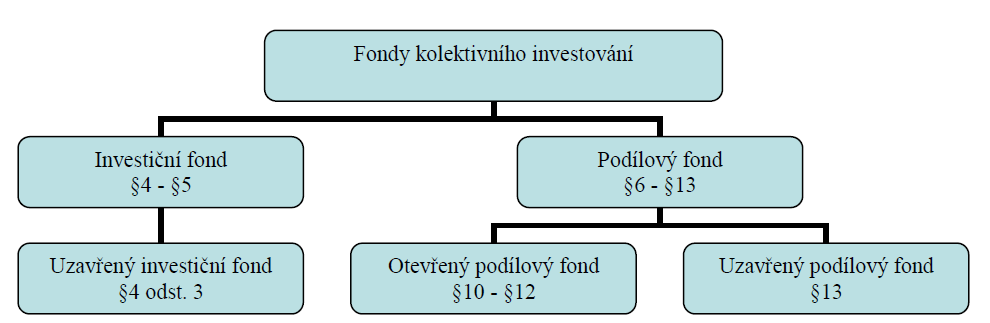
\includegraphics[width=\textwidth]{deleni.png}
\caption{Členění fondů kolektivního investování dle zákona č. 189/2004 Sb., o kolektivním investování, zdroj: \cite{dp}}
\end{figure}

Podle práva na zpětný odkup podílových listů dělíme podílové fondy na otevřené a uzavřené.

\emph{Otevřený podílový fond} má povinnost zpětného odkupu podílových listů za aktuální hodnotu na základě žádosti podílníka, a to nejpozději do 15 pracovních dní od podání žádosti. Otevřený fond nemá předem omezen počet emitovaných podílových listů, nemá tedy omezen počet podílníků.

\emph{Uzavřený podílový fond} má již při svém vzniku stanoven počet podílových listů, které může emitovat. Je zakládán na dobu určitou, po této době vstupuje do likvidace, anebo se změní na otevřený fond.



\newpage

\renewcommand{\refname}{Seznam použité literatury}
\begin{thebibliography}{9}
\addcontentsline{toc}{section}{Seznam použité literatury}
\thispagestyle{plain}
\bibitem{zakon} Zákon č. 189/2004 Sb., o kolektivním investování
\bibitem{zafi} SVOBODA, Martin. \emph{Základy financí.} 1. vyd. Brno: Masarykova univerzita, 2009, 195 s. ISBN 978-802-1049-765. 
\bibitem{dp} VAŠKOVÁ, Lucie. \emph{Kolektivní investování v České republice.} Brno, 2011. Dostupné z: \url{http://is.muni.cz/th/206629/esf_m/}. Diplomová práce. Masarykova univerzita, Ekonomicko-správní fakulta. Vedoucí práce Ing. Dalibor Pánek.
\end{thebibliography}
\end{document}

\end{document}